%! Author = emile
%! Date = 28/05/2020

% Preamble
\documentclass[11pt]{article}

% Packages
\usepackage{tikz}
\usepackage{amsmath}
\usetikzlibrary{arrows,topaths,shapes.geometric, positioning}

\tikzstyle{tikzdet} = [rectangle, minimum width=1cm, minimum height=1cm,text centered, draw=black]
\tikzstyle{tikzstoch} = [ellipse, align=center, minimum width=1cm, minimum height=1cm,text centered, draw=black]
\tikzstyle{tikzparam} = [rectangle, align=center, minimum width=0cm, minimum height=0cm,text centered, draw=white]

% Document
\begin{document}

%\begin{tikzpicture}[node distance=1cm]
%    \node (a)  [tikzparam] {$a$};
%    \node (b)  [tikzparam, below of=a] {$b$};
%    \node (c)  [tikzparam, below of=b] {$c$};
%    \node (ab) [tikzdet, right=1cm of a] {$d=a+b$};
%%    \node (bc) [tikzdet, right=1cm of c] {$e=c+b$};
%    \node (bc) [tikzstoch, right=1cm of c] {$e\sim$ \\ $ \mathcal{N}(c+b, 1)$};
%    \node (abc) [tikzdet, right=4cm of b] {$f=d * e$};
%
%    \draw [->] (a) -- (ab);
%    \draw [->] (b) -- (ab);
%    \draw [->] (c) -- (bc);
%    \draw [->] (b) -- (bc);
%    \draw [->] (ab) -- (abc);
%    \draw [->] (bc) -- (abc);
%\end{tikzpicture}

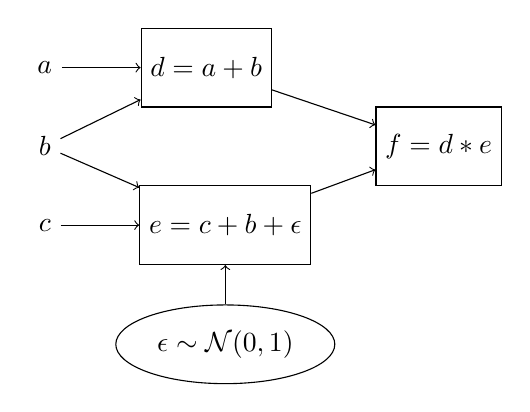
\begin{tikzpicture}[node distance=1cm]
    \node (a)  [tikzparam] {$a$};
    \node (b)  [tikzparam, below of=a] {$b$};
    \node (c)  [tikzparam, below of=b] {$c$};
    \node (ab) [tikzdet, right=1cm of a] {$d=a+b$};
    \node (bc) [tikzdet, right=1cm of c] {$e=c+b + \epsilon$};
    \node (eps) [tikzstoch, below=0.5cm of bc] {$\epsilon\sim \mathcal{N}(0, 1)$};
    \node (abc) [tikzdet, right=4cm of b] {$f=d * e$};

    \draw [->] (a) -- (ab);
    \draw [->] (b) -- (ab);
    \draw [->] (c) -- (bc);
    \draw [->] (b) -- (bc);
    \draw [->] (ab) -- (abc);
    \draw [->] (bc) -- (abc);
    \draw [->] (eps) -- (bc);
\end{tikzpicture}

\end{document}